\documentclass[a4paper]{article}

\usepackage[english]{babel}
\usepackage[utf8]{inputenc}
\usepackage{apacite}
\usepackage{graphicx}
\usepackage{tikz}
\usetikzlibrary{positioning}
\usepackage{xcolor}
\usepackage[colorinlistoftodos]{todonotes}

\makeatletter
\def\BState{\State\hskip-\ALG@thistlm}
\makeatother

\title{Gameplay Design \\ Assignment 2 }

\author{
  Bowald, Johan\\
  \texttt{bowaldj@student.chalmers.se}
  \and
  Odbjer, Sebastian\\
  \texttt{sebastian.odbjer@gmail.com}
}

\date{\today}

\tikzset{
    vertex/.style = {
        circle,
        fill  = black,
        outer sep = 2pt,
        inner sep = 1pt,
    }
}

\begin{document}
\maketitle
\newpage
\tableofcontents{}

\section{Introduction}

\section{Gameplay description 7 wonders}

\subsection{What is 7 wonders?}
7 wonder was released in 2010 and the goal is to build a civilisation in an ancient setting. 
The game consist of several card types and a player unique game board showing the status of a players civilisation. The different cards represents different buildings which each contribute to the civilisation in some way. There are resource spawning, such as iron, chemicals or wood. Military cards which are used to battle with one's neighbours, these battles gives points to the victor and minus point to the defeated one. Battles is Science Cards, which generate points at the end of the game, the amount of points is based on the amount of science tool sets collected and the number of each science tool.
Another card type is what we have called utility cards, they have an immediate effect on the game state, these are cards that either is tradeable for currency or trading posts that gives discount for trading with one's neighbours. Last card type is point cards, either buildings that gives a fixed amount of points or dynamic point cards that is based on oneself civilisation status or ones neighbours statuses. The game is divided into three ages, each age is divided into six turns. Each turn, each player picks a card which is either played, discarded or used as a resource to build a wonder. The rest of the cards is passed to the next player in a drafting fashion. To play a card some resources must be paid, they can either be resources generated Wonders have different impact on the game, they can either generate resources, points, currency or military power. The effect of wonders are unique for each civilisation. After the three ages points are counted for each player based on each card type, and the amount of currency when the game is over. The player that has the most point at the end wins the game. 

\subsection{Thoughts on gameplay of 7 wonders}
The gameplay in this game is centered around the draft mechanic. A player will always consider wich strategy to use based on his neighbours choice of card, what resources he has 

Boardgamegeeks REF characterize it as a strategy game while criticalboardgamer characterize it as a Drafting game. Neither is contradicts each other but one could argue that the characteristics of a drafting game could be more explanatory for the game play in the game.

7 wonders can be played with two to seven player. Boardgamegeeks suggest that its best with four players. The argument is that since each player only can have two neighbors  

\subsection{7 wonders analysis using game design patterns}
\begin{figure}

\centering
  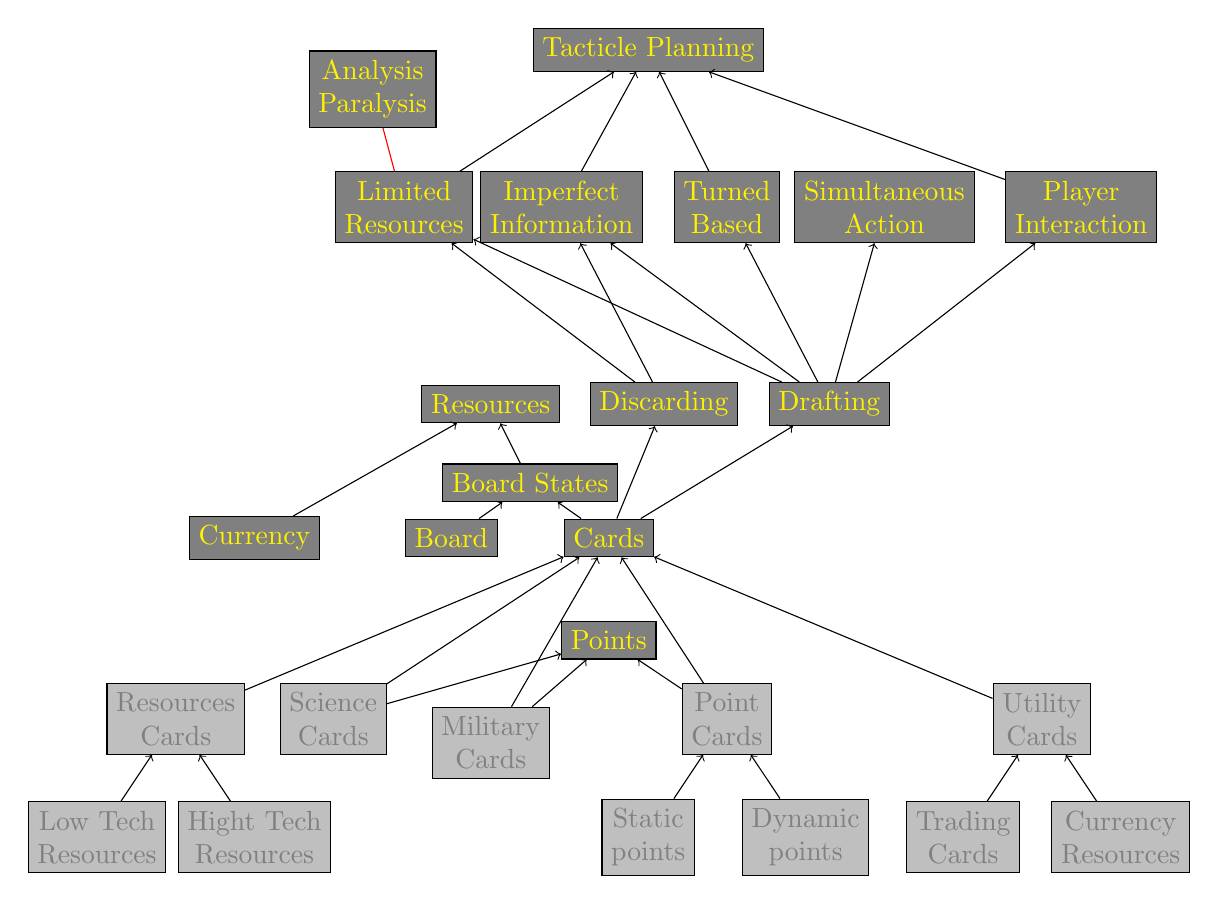
\begin{tikzpicture}

  \node[draw,fill=gray!50,text=gray, align=center] (LTRe) at (-6,0) {Low Tech\\ Resources};
  \node[draw,fill=gray!50,text=gray, align=center] (HTRe) at (-4,0){Hight Tech\\ Resources};

  \node[draw,fill=gray!50,text=gray, align=center] (CuRe) at (7,0) {Currency \\Resources};
  \node[draw,fill=gray!50,text=gray, align=center] (TrCa) at (5,0) {Trading \\Cards};  

  \node[draw,fill=gray!50,text=gray, align=center] (StPo) at (1,0) {Static\\points};
  \node[draw,fill=gray!50,text=gray, align=center] (DyPo) at (3,0) {Dynamic\\points};
  
  \node[draw,fill=gray!50,text=gray, align=center] (ReCa) at (-5,1.5) {Resources\\ Cards};
  \draw[->,draw=black] (LTRe) to (ReCa);
  \draw[->,draw=black] (HTRe) to (ReCa);
  \node[draw,fill=gray!50,text=gray, align=center] (ScCa) at (-3,1.5) {Science\\Cards};
  \node[draw,fill=gray!50,text=gray, align=center] (MiCa) at (-1,1.2) {Military\\Cards};
  \node[draw,fill=gray!50,text=gray, align=center] (PoCa) at (2,1.5) {Point\\Cards};
  \draw[->,draw=black] (DyPo) to (PoCa);
  \draw[->,draw=black] (StPo) to (PoCa);
  \node[draw,fill=gray!50,text=gray, align=center] (UtCa) at (6,1.5) {Utility\\Cards};
  \draw[->,draw=black] (TrCa) to (UtCa);
  \draw[->,draw=black] (CuRe) to (UtCa);

  \node[draw,fill=gray,text=yellow] (Po) at (0.5,2.5) {Points};

  \draw[->,draw=black] (ScCa) to (Po);
  \draw[->,draw=black] (MiCa) to (Po);
  \draw[->,draw=black] (PoCa) to (Po);

  \node[draw,fill=gray,text=yellow] (Ca) at (0.5,3.8) {Cards};

  \draw[->,draw=black] (ScCa) to (Ca);
  \draw[->,draw=black] (MiCa) to (Ca);
  \draw[->,draw=black] (PoCa) to (Ca);
  \draw[->,draw=black] (ReCa) to (Ca);
  \draw[->,draw=black] (UtCa) to (Ca);
  
  % \node[draw,fill=gray!50,text=gray, align=center ](PoTo) {Point\\Tokens};
  \node[draw,fill=gray,text=yellow] (Cu) at (-4,3.8){Currency};
  \node[draw,fill=gray,text=yellow] (Bo) at (-1.5,3.8){Board};


  % %to points, resouces
  \node[draw,fill=gray,text=yellow] (BoSt) at (-0.5,4.5) {Board States};
  \draw[->,draw=black] (Bo) to (BoSt);
  \draw[->,draw=black] (Ca) to (BoSt);

  \node[draw,fill=gray,text=yellow] (Re) at (-1,5.5) {Resources};
  \node[draw,fill=gray,text=yellow] (Di) at (1.2,5.5) {Discarding};
  \node[draw,fill=gray,text=yellow] (Da) at (3.3,5.5) {Drafting};
  \draw[->,draw=black] (Cu) to (Re);
  \draw[->,draw=black] (BoSt) to (Re);
  \draw[->,draw=black] (Ca) to (Da);
  \draw[->,draw=black] (Ca) to (Di);

  % %Drafting, discarding
  \node[draw,fill=gray,text=yellow, align=center] (ImIn) at (-0.1,8) {Imperfect\\Information};
  \node[draw,fill=gray,text=yellow, align=center] (LiRe) at (-2.1,8) {Limited\\Resources};
  \node[draw,fill=gray,text=yellow, align=center] (TuBa) at (2,8) {Turned\\Based};
  \node[draw,fill=gray,text=yellow, align=center] (SiAc) at (4,8) {Simultaneous\\Action};
  \node[draw,fill=gray,text=yellow, align=center] (PlIn) at (6.5,8) {Player\\Interaction};

  \draw[->,draw=black] (Di) to (ImIn);
  \draw[->,draw=black] (Di) to (LiRe);

  \draw[->,draw=black] (Da) to (ImIn);
  \draw[->,draw=black] (Da) to (LiRe);
  \draw[->,draw=black] (Da) to (TuBa);
  \draw[->,draw=black] (Da) to (SiAc);
  \draw[->,draw=black] (Da) to (PlIn);

  % %Drafting trading cards
  
  \node[draw,fill=gray,text=yellow, align=center] (AnPa) at (-2.5,9.5){Analysis\\Paralysis};
  \draw[-,draw=red] (LiRe) to (AnPa);
  \node[draw,fill=gray,text=yellow] (TaPl) at (1,10){Tacticle Planning};
  \draw[->,draw=black] (ImIn) to (TaPl);
  \draw[->,draw=black] (LiRe) to (TaPl);
  \draw[->,draw=black] (TuBa) to (TaPl);
  \draw[->,draw=black] (PlIn) to (TaPl);

  % \node[draw,fill=gray,text=yellow] (KiMa) {King Maker};

  \end{tikzpicture}
\caption{Analysis of 7 Wonders using Game Design Pattern}
\label{fig:A7W}
\end{figure}

\
\section{Gameplay description Richoceting Robots}
\subsection{What is Richocheting Robots?}
Ricochet robots is a game where players challenge each other to move a robot to a certain point.. The game consists of a board with a grid layout. Some of the grid tiles are unique goal tile. The goal tiles have a color matching one of the robots(except the optional support robot) and a symbol. The board also have walls placed between some tiles. A robot cannot move through these walls, instead they ricochet along the wall in the direction of the players choice. Each turn a goal token is revealed and each player simentainusly tries to figure out the path with the fewest moves to take the robot with the matching color as the goal token to the goal tile with the same symbol and color as the goal token. 

, with the goal of move a specific robot from one point to a goal point. When one player have found a legit path, that player state the amount of movements required to carry out the task. The other players have one minute to try to beat the first player number of movements. When the time ends, that player with the fewest movements gets the point and a new turn begins. When all goal tokens are collected by the players, the player with the most goal tokens wins the game.

\subsection{Thoughts on gameplay of Richocheting Robots}

\subsection{Ricocheting Robots analyzed using Game Design Patterns}
% Ricocheting Robots Game pettern analysis
\begin{figure}
\centering
  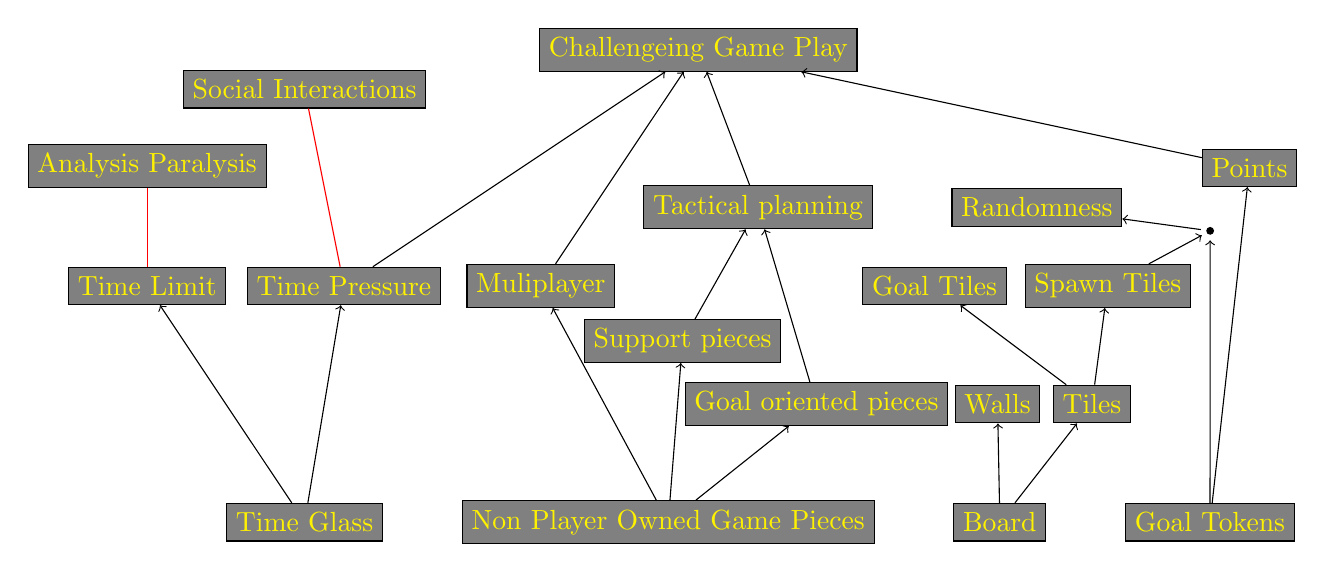
\begin{tikzpicture}
    \node[draw,fill=gray,text=yellow] (TimeGlass) at (-5,0) {Time Glass};
    \node[draw,fill=gray,text=yellow, right=of TimeGlass] (NPGP) {Non Player Owned Game Pieces};
    \node[draw,fill=gray,text=yellow, right=of NPGP] (Board) {Board};
    \node[draw,fill=gray,text=yellow, right=of Board] (GoalTokens) {Goal Tokens};

    \node[draw,fill=gray,text=yellow] at (1.5,1.5) (GoalP) {Goal oriented pieces};  
    \node[draw,fill=gray,text=yellow] at (-0.2,2.3) (SP) {Support pieces};  
    \node[draw,fill=gray,text=yellow] (Walls) at (3.8,1.5) {Walls};  
    \node[draw,fill=gray,text=yellow] (Tiles) at (5,1.5) {Tiles};  

    \node[draw,fill=gray,text=yellow] (TimeLimit) at (-7, 3) {Time Limit};  
    \node[draw,fill=gray,text=yellow] (TimeP) at (-4.5, 3) {Time Pressure};  
    \node[draw,fill=gray,text=yellow] (SI) at (-5, 5.5){Social Interactions};

    \node[draw,fill=gray,text=yellow] (MP) at (-2, 3){Muliplayer};

    \node[draw,fill=gray,text=yellow] (SpawnT) at (5.2,3) {Spawn Tiles};  
    \node[draw,fill=gray,text=yellow] (GoalT)  at (3,3) {Goal Tiles};  

    \node[draw,fill=gray,text=yellow] (Randomness) at (4.3,4){Randomness};
    \node[draw,fill=gray,text=yellow, left=of Randomness] (TacP) {Tactical planning};  
    \node[draw,fill=gray,text=yellow] (Points) at (7,4.5) {Points};
    \node[draw,fill=gray,text=yellow, above=of TimeLimit] (AP) {Analysis Paralysis};
    \node[draw,fill=gray,text=yellow] (CGP) at (0,6) {Challengeing Game Play};

    \draw node[vertex] (JointGT) at (6.5,3.7) {};

    \draw[->,draw=black] (TimeGlass) to (TimeLimit);
    \draw[->,draw=black] (TimeGlass) to (TimeP);

    \draw[->,draw=black] (NPGP) to (GoalP);
    \draw[->,draw=black] (NPGP) to (SP);
    \draw[->,draw=black] (Board) to (Walls);
    \draw[->,draw=black] (Board) to (Tiles);  

    \draw[->,draw=black] (GoalTokens) to (JointGT);
    \draw[->,draw=black] (SpawnT) to (JointGT);
    \draw[->,draw=black] (GoalTokens) to (Points);
    \draw[->,draw=black] (JointGT) to (Randomness);

    \draw[->,draw=black] (Tiles) to (SpawnT);
    \draw[->,draw=black] (Tiles) to (GoalT);
    \draw[->,draw=black] (NPGP) to (MP);
    \draw[->,draw=black] (MP) to (CGP);
    \draw[->,draw=black] (TimeP) to (CGP);
    \draw[->,draw=black] (Points) to (CGP);
    \draw[->,draw=black] (TacP) to (CGP);
    \draw[->,draw=black] (SP) to (TacP);
    \draw[->,draw=black] (GoalP) to (TacP);


    \draw[-,draw=red] (TimeLimit) to (AP);
    \draw[-,draw=red] (TimeP) to (SI);

  \end{tikzpicture}

  \caption{Analysis of Richocheting Robots using Game Design Pattern} 
  \label{fig:RRW}
\end{figure}

\section{Similarities and difference between the game using our analysis}
  Här kan vi dra slutsater om likheter och olikheter baserat på analysen mha Game design patterns. 

\section{Design structures in the games}
Short description on what we are looking for

\subsection{Design structures used to keep players engaged with the game}
\paragraph{7 Wonders} is made out of turns but all players are playing at the same time. The state of the gameboard are always change so one needs to pay attention of during each round. Since the game offers a lot of ways to collect points one could always change their current strategy to get back in the game, to retain their interest.

\paragraph{In Ricocheting Robots} everyone is playing simultaneously often you can not be sure that you have found an optimal solution, therefore a player can always try to find a better solution. Intense Competitive game play due to the time stress. If someone is dominating their opponents, the game session is so short that players are probably not losing their interests.

\subsection{Design structures used to make the games typically end near the state time}
\paragraph{7 Wonders} have a fixed amount of cards to play during each of the three stages of the game. One card is played each round and each stage consists of six rounds.

\paragraph{Ricocheting Robots} ha a limited number of Goal tokens, which regulate the game time. There is a possibility that the game end before all tokens are used, since a player only need to collect a constant number of tokens to win the game.

\subsection{Design structures used to make players interact with each other}

\paragraph{In 7 wonders} your strategy are both dependent on the cards you are given and the strategy your opponents choose.

\paragraph{In Ricocheting Robots} the players are always trying to beat their own or other players solutions, by figure out another one path to the goal using even fewer moves. Wich means that the player interaction is the bread and butter of the game design, since the difficulty of the game is based on cost of the current known best paths, which is always stated by a player.

\subsection{Design structures to make players feel that they are achieving something}
\paragraph{7 wonders} gives the player the ability to build a civilisation. Even if the player indirectly are collecting points by building theese aspects of the civilisation. When the game ends each players civilisation have made a giant leap in progress then when the game started.

\paragraph{In Ricocheting Robots} when a player found a path he had achived something. Even if is not the winning path, a player still has figured out the puzzle.

\section{What parts of the gameplay are missing or unfun?}


\newpage
\bibliographystyle{apacite}
\bibliography{bib}

\end{document} 

